\documentclass[12pt]{article}

% For formatting
\usepackage[margin=1truein]{geometry}
\usepackage{fancyhdr}
\usepackage{setspace}
\usepackage{titlesec}
\usepackage{graphicx}
\usepackage{float}
\usepackage{indentfirst}

\usepackage[style=apa, backend=biber]{biblatex}
\addbibresource{refs.bib}

% Font
\usepackage{newtxtext}
\usepackage[bigger]{musicography}
\usepackage{amsmath}


% For starting the page number on the title page
\usepackage{etoolbox}
\patchcmd{\titlepage}
    {\thispagestyle{empty}}
    {\thispagestyle{fancy}}
    {}
    {}

\titleformat*{\section}{\centering\normalsize\bfseries}
\titlespacing*{\section}{0pt}{0pt}{0pt}
\titleformat*{\subsection}{\normalsize\bfseries}
\titlespacing*{\subsection}{0pt}{0pt}{0pt}
\titleformat*{\subsubsection}{\normalsize\bfseries\itshape}
\titlespacing*{\subsubsection}{0pt}{0pt}{0pt}

\newcommand{\mytitle}{A Naive Morphology of Harmonic Analysis}

\pagestyle{fancy}
\fancyhf{}
\fancyhead[R]{\thepage}
\renewcommand{\headrulewidth}{0pt}
\setlength{\headheight}{15pt}

\onehalfspacing
\begin{document}
    \begin{titlepage}
  \begin{center}
    {\doublespacing
      \vspace*{4\baselineskip}

      \textbf{\mytitle}
      \vspace*{\baselineskip}

      Jaden Nola

      Department of English, Wichita State University

      LING 151: Nature of Language

      Kaitlyn Hemberger

      May 4, 2023\par
    }
  \end{center}
\end{titlepage}

    \setcounter{page}{2}
    {\centering
      \textbf{\mytitle}\par
    }
    \textit{Notes} are a convention used to classify musical pitch. An octave
    is the interval between a pitch and another pitch with double its 
    frequency. Notes, then, are defined as the 12 equidistant frequencies within
    an octave, excluding the top boundary. In the system used by Western art
    music, called \textit{12-tone equal temperament}, the note A is defined to
    be 440~Hz, and the other notes follow from this assumption. In order of
    increasing pitch, they are
    A,~A\sh,~B,~C,~C\sh,~D,~D\sh,~E,~F,~F\sh,~G,~and~G\sh. This sequence
    repeats, meaning the note that follows G\sh{} would be A\@. The \sh{}
    symbol implies being higher pitched than the note it is modifying,
    but it is also possible to denote being of lower pitch using the \fl{}
    symbol. Thus, the notes can also be written as:
    A,~B\fl,~B,~C,~D\fl,~D,~E\fl,~E,~F,~G\fl,~G,~and~A\fl. Of course, the
    highest note of this sequence does not have a lower pitch than the first
    note of the sequence but rather lower than the note an octave above the
    first note of the sequence. We should also note that note names are not
    unique, as we can classify C to be B\sh{} or B to be C\fl, but these
    conventions are for specialized cases out of the scope of this paper.

    A combination of notes played together is called a \textit{chord}. Chords
    are native to a key signature, which are defined by the spaces between
    consecutive notes. The major key signature is defined by the spaces
    2-2-1-2-2-2-1, so C major would be the notes C-D-E-F-G-A-B\@. The minor
    key signature, on the other hand, is defined by 2-1-2-2-1-2-2; thus, C
    minor is C-D-E\fl-F-G-A\fl-B\fl. We use roman numerals to label a special
    type of chord with three notes, where all are one note away from each
    other within the key signature. In C major, (\RN{1}) is the chord C-E-G,
    and (\Rn{2}) is D-F-A\@. (\Rn{2}) is lowercase because it corresponds to
    the (\Rn{1}) chord in D minor. This is to say that the chords in C major
    are (\RN{1})-(\Rn{2})-(\Rn{3})-(\RN{4})-(\RN{5})-(\Rn{6})-(\Rn{7}\textsuperscript{o})
    and in C minor are
    (\Rn{1})-(\Rn{2}\textsuperscript{o})-(\RN{3})-(\Rn{4})-(\Rn{5})-(\RN{6})-(\RN{7}).
    When we want to reference specific chords rather than their position, we
    use capital letters; thus, in C major, the chords are C-Dm-Em-F-G-Am-Bdim,
    where "m" signifies a minor chord and "dim" signifies a diminished chord,
    a chord containing the note six steps above the base note. 
    \section*{Research Question}
    {\centering
        How can aspects of morphology be applied to four-part diatonic
        harmony?\par
    }
    \section*{Methodology}
    We will mainly base our observations in the key of C major in order to
    simplify and shorten our analysis, but this process can be repeated for
    any key. In a loose sense, we will take notes to be analogous to phonemes
    or allophones, chords to morphemes, and chord progressions to be
    sentences. With this assumption in mind, we will analyze chords and their
    purposes in chord progressions. More specifically, we will be analyzing
    the word order and processes of word formation in harmony involving
    three to four voices or instruments.
    \section*{Results and Discussion}
    \subsection*{Word Order}
    \textcite{schoenberg_1969} categorizes chords into three functions:
    tonic (T), succession (S), and progression (P). For simplicity, we will 
    think of each as the following: tonic chords are the place of least 
    tension, succession chords create tension, and progression chords are the
    place of most tension with the intent of returning to a tonic chord. With
    this method of labeling, we deduce that the dominant word order is TSPT\@.
    To clarify, we will analyze the chord progression in
    Figure~\ref{fig:c_perf_cad}, called a perfect cadence.
    \begin{figure}[H]
        \centering
        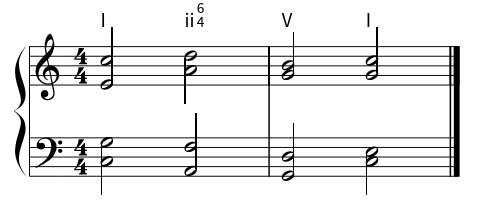
\includegraphics[width=0.5\linewidth]{1-2-5-1-demo.png}
        \caption{A perfect cadence in C major (with sub-par voice leading, by the author)}
        \label{fig:c_perf_cad}
    \end{figure}
    The perfect cadence, the sequence of (I)-(ii)-(V)-(I), in C major is
    C-Dm-G-C\@. If this follows our supposed word order, we find that C is a
    tonic chord, Dm is a succession chord, and G is a progression chord, but
    what justifies this? It makes sense that C is a tonic chord since we are
    in the key of C major. We will motivate the purpose of Dm by first
    analyzing the purpose of G\@. G is composed of G-B-D, and C is composed of
    C-E-G, so they have one note in common. However, we should also note that
    the notes B and D are one and two spaces away from C and E, respectively. 
    Because we are in the key of C major, they both \textit{really} want to
    resolve to the notes of the tonic chord. In fact, this is true for the (V)
    chord of any major key signature. Armed with this knowledge, we can then
    analyze Dm from the perspective of the key signature of G major. Although
    G major has the chord D rather than Dm, the same principles apply and Dm
    wants to resolve to G, but since Dm is being used to get to G rather than
    C, it is a succession chord. The principles discussed here can be applied
    to any key signature, thus being true for the more general
    (I)-(ii)-(V)-(I) cadence.

    Near the end of the last paragraph, it was hinted at that a single chord
    serve multiple functions, making it possible to be tonic, successive, or
    progressive. In general, a chord's function is defined by the context of
    the chord progression. Lastly, we will note that composers may subvert the
    audience's expectations of resolution (i.e., (V)-(I) as discussed above)
    to produce a desired effect, similar to word play in comedy. This allows
    us to conclude that word order in music is extremely flexible.
    \subsection*{Word Formation Processes}
    \subsubsection*{Derivation}
    Derivation is the process of creating new words from existing words, which
    do not have to be the same part of speech as the original 
    word~\autocite[p.~36]{jackson_stockwell_2011}. We can replicate this same
    process by adding more notes to existing chords, such as adding the note
    D to the chord C, giving the notes C-D-E-G\@. Now instead of being a chord
    of least tension, this chord, named Csus2, provides some tension to
    resolve back to the regular C chord, but not as much as the progressive
    chord G\@. As expected, adding this note has changed the function of the
    chord and is an example of morphological derivation in harmony.
    \subsubsection*{Inflection}
    While inflection is very similar to derivation, it is different in that
    the part of speech stays the same and it expresses some grammatical
    category~\autocite[p.~36]{jackson_stockwell_2011}. The musical equivalent
    of inflection would be chord \textit{inversion}, the permutation of notes
    in a chord. As of now, we ordered the notes from lowest to highest pitch,
    so the notes in Dm were D-F-A, but we can permute them to be A-D-F, as
    seen in Figure~\ref{fig:c_perf_cad} denoted by the superscript 6 and 4.
    These inversions influence where a chord wants to resolve. For example,
    Bdim, or (vii\textsuperscript{o}) in C major, is a progressive chord that
    wants to resolve to the chord C; however in the key signature of B\fl{}
    major, Bdim is a non-diatonic (not belonging to the key) chord that wants
    to resolve to the chord B\fl. In root position B-D-F, the chord wants to
    resolve to G-C-E, the chord C or ($\text{I}^{{}^6_4}$), but in second
    inversion F-B-D, it wants to resolve to F-B\fl-D, the chord B\fl{} or
    also ($\text{I}^{{}^6_4}$) in the key B\fl{} major. This is to say,
    chord inversion keeps the function or part of speech of a chord the same,
    but gives directionality.
    \subsubsection*{Reduplication}
    Reduplication consists of reduplicating all or some morphemes to make new
    words~\autocite[p.~168]{dawson_phelan_2016}. While adding notes to chords
    is more like adding an analogue of phonemes, we can still observe the
    morphological changes that come with duplicating existing notes.
    Duplicating the root of a chord increases its stability, so the C chord
    would become C-E-G-C, a chord of even less tension. In general, doubling
    any of the other notes creates even more tension and instability, which
    urges the chord progression to move along, especially when doubling the
    note seven spaces above the root, known as the fifth.
    \subsubsection*{Compounding}
    Compounding is the combination of two or more free morphemes, which can
    stand alone without attachment, to make a new 
    word~\autocite[p.~166]{dawson_phelan_2016}. This effect can be seen in
    polychords, the stacking of two or more chords. For example, a polychord
    of C and D would be made up of the notes C-E-G-D-F\sh-A, notated
    \(\frac{\text{I}}{\text{II}}\) in C major. This will be the extent of the
    discussion for polychords as this paper focuses on diatonic harmony.
    \newpage
    \printbibliography
\end{document}
